\documentclass[11pt]{article}

% ==========================
% ESSENTIAL PACKAGES
% ==========================
\usepackage[utf8]{inputenc}  % Character encoding
\usepackage[T1]{fontenc}     % Font encoding
\usepackage[english]{babel}  % Document language
\usepackage{csquotes}        % Support for quotations

% ==========================
% FORMATTING & STRUCTURE PACKAGES
% ==========================
\usepackage[dvipsnames]{xcolor} % Advanced colors
\usepackage{graphicx}           % Image handling
\usepackage{subcaption}         % Subcaptions for images
\usepackage{fancyhdr}           % Custom headers & footers
\usepackage{vmargin}            % Custom margins
\usepackage{hyperref}           % Clickable links
\usepackage{booktabs}           % Professional tables
\usepackage{amsmath}            % Math symbols & equations
\usepackage{wrapfig}            % Wrapping text around figures
\usepackage{soul}               % Underlining and highlighting
\usepackage{float}              % Better float positioning
\usepackage{tcolorbox}          % Colored boxes for highlights
\usepackage{verbatim}           % Multi-line comments
\usepackage{cclicenses}
\usepackage{titlesec}
\usepackage{enumitem}

\newcommand{\sectionbreak}{\clearpage}
\titleformat{\section}[block]{\huge\bfseries}{\thesection.}{1em}{}
\setlength{\parskip}{0.7em}
\setlist{itemsep=0.2em, topsep=0.2em}

% ==========================
% BIBLIOGRAPHY CONFIGURATION
% ==========================
\usepackage{biblatex}  % Bibliography management
\addbibresource{biblio.bib}  % Reference to the .bib file

% ==========================
% TABLE OF CONTENTS & SECTION DEPTH
% ==========================
\setcounter{tocdepth}{5}  % Depth of table of contents
\setcounter{secnumdepth}{2}  % Depth of numbered sections

% ==========================
% MARGINS CONFIGURATION
% ==========================
\setmarginsrb{2.5cm}{2.5cm}{2.5cm}{2.5cm}{1cm}{1.5cm}{1cm}{1.5cm}
\graphicspath{{./images/}}

% ==========================
% TITLE PAGE CONFIGURATION
% ==========================
\newcommand{\ctitle}{Emulating the NXP S32K3X8EVB in QEMU \& Porting FreeRTOS}
\title{\ctitle}

%Emulation of the NXP S32K3X8EVB in QEMU and Porting of FreeRTOS%
%TITOLO SOSTITUTIVO%

\author{} % Left empty as authors will be manually added below
\date{February 18, 2025}

\makeatletter
\let\thetitle\@title
\let\theauthor\@author
\let\thedate\@date
\makeatother

% ==========================
% PDF METADATA & FOOTER CONFIGURATION
% ==========================
\hypersetup{
    pdftitle={\thetitle},
    pdfsubject={},
    pdfkeywords={},
    hidelinks
}
\pagestyle{fancy}
\fancyhf{}
\fancyfoot[L]{\ccnc CC BY-NC 4.0 | Politecnico di Torino - CAOS group 18 2024/2025}
\fancyfoot[R]{\thepage} 
\fancyhead[L]{\ctitle}

\fancypagestyle{plain}{
    \fancyhf{}
    \fancyfoot[L]{\ccnc CC BY-NC 4.0 | Politecnico di Torino - CAOS group 18 2024/2025}
    \fancyfoot[R]{\thepage} 
    \fancyhead[L]{\ctitle}
}

\begin{document}

% ==========================
% TITLE PAGE
% ==========================
\begin{titlepage}
    \centering
    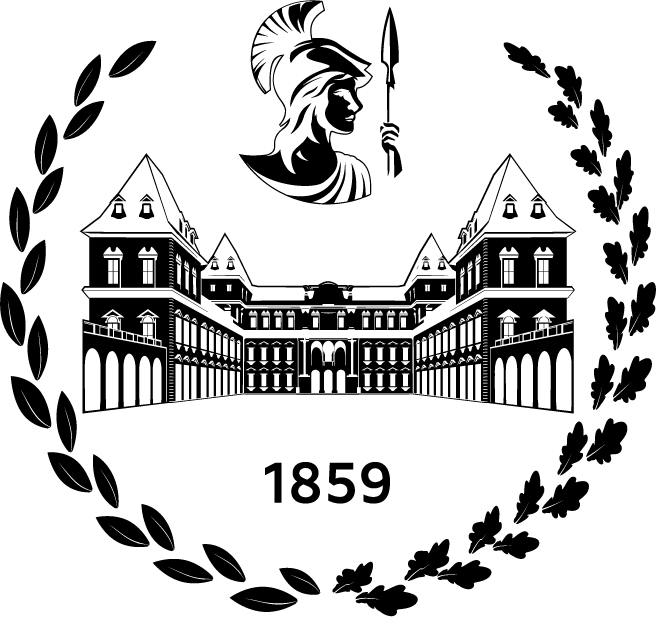
\includegraphics[scale=0.4]{logoPoli.png}\\[1.0 cm]
    \textsc{\LARGE POLITECNICO DI TORINO}\\[0.2 cm]
    \textsc{\large Master’s Degree in Cybersecurity}\\[4 cm]
    {\huge \bfseries \ctitle}\\[0.2 cm]
    \rule{0.6\linewidth}{0.25 mm}\\[0.3 cm]
    \textsc{\Large CAOS Project Report}\\[0.7 cm]

    \vspace{2cm} % Space before authors section

    \begin{flushleft} \large
        \textbf{Authors:}\\[0.1cm]
        Group 18 2024/2025\\[0.1cm]
        Bertolami Carmelo - s345963\\[0.1cm]
        Frigo Matteo - s338605\\[0.1cm]
        Simoncini Marco - s341631\\[0.1cm]
        Soldera Marco - s338823
    \end{flushleft}

    \vfill
\end{titlepage}

{\centering \Huge \textbf{License} \par}
\vspace{1cm} % Adds space between title and text
\noindent This work is licensed under a Creative Commons Attribution-NonCommercial 4.0 International License. \newline
\url{http://creativecommons.org/licenses/by-nc/4.0/}
\pagebreak

% ==========================
% TABLE OF CONTENTS
% ==========================
\include{ext_sections/preliminary}
\include{ext_sections/contributors}
\tableofcontents
\pagebreak

% ==========================
% CHAPTERS
% ==========================
\section{Introduction}

This document describes the work carried out within the course of \textbf{Computer Architecture and Operating Systems}, with the aim of developing skills in the emulation of heterogeneous hardware architectures using \textbf{QEMU}, porting the \textbf{FreeRTOS} operating system, and collaboratively managing code through \textbf{Git}.

\noindent The project is divided into three main phases:
\begin{itemize}
    \item \textbf{Emulation of a board in QEMU}: Implementation of support for the \textbf{NXP S32K3X8EVB} board, including CPU, memory mapping, and UART and CAN drivers.
    \item \textbf{Porting of FreeRTOS}: Verification of the correct functioning of the operating system in the emulated environment.
    \item \textbf{Development of a test application}: Implementation of a multitasking application to validate the emulation.
\end{itemize}

Everything has been implemented and developed within a GitLab repository, a process that required careful collaboration and constant team coordination.

The objective of this document is to provide a detailed technical description of the implementation process, illustrating the design choices adopted, the challenges encountered, and the solutions implemented.

Furthermore, the \textbf{README} files in GitLab provide instructions for compilation, execution, and testing of the emulated environment.


\section{NXP S32K3X8EVB Board Description}

The \textbf{NXP S32K3X8EVB} \cite{nxp_s32k3x8evb} is an Evaluation Board designed for the development of automotive applications. This board is based on the \textbf{S32K358} microcontroller, which belongs to the \textbf{S32K3} family. It supports applications requiring functional safety, advanced communications, and efficient hardware resource management. The following are some of its key technical specifications.

\subsection{Main Components}
\label{sec:components}

The \textbf{SoC} that is present in the board is S32K358. It integrates all the main components of the board. On this specific SoC there is a CPU with the following specifications:
\begin{itemize}
    \item \textbf{ARM Cortex-M7} CPU 32-bit architecture.
    \item Maximum frequency: up to \textbf{320 MHz}.
\end{itemize}
The \textbf{memory} of this SoC is divided many minor sections that resulted not useful for the purpose of emulation and the following five main sections:
\begin{itemize}
    \item Program Flash as \textbf{ROM}: \textbf{8 MB}.
    \item Data Flash as \textbf{ROM}: \textbf{128 KB}.
    \item ITCM as \textbf{RAM}: \textbf{32 KB}.
    \item DTCM as \textbf{RAM}: \textbf{64 KB}.
    \item \textbf{3 SRAM regions} of \textbf{256 KB} each.
\end{itemize}
The board has multiple \textbf{communication interfaces} to interact with sensors and other devices:
\begin{itemize}
    \item \textbf{CAN-FD} (Controller Area Network with Flexible Data Rate) for high-speed automotive communication.
    \item \textbf{UART, SPI, I2C} for standard serial communications.
\end{itemize}

\subsection{Project Context}
In the context of this project, we will limit the emulation to the following components:
\begin{itemize}
    \item \textbf{SoC S32K358};
    \item \textbf{ARM Cortex-M7 CPU} (already in Qemu);
    \item \textbf{Memory} structure emulation;
    \item \textbf{UART} emulation and communication;
    \item \textbf{CAN} emulation and communication through CAN bus.
\end{itemize}
\section{Qemu implementation}
QEMU \cite{qemu_documentation} is an open-source emulator and virtualizer that allows operating systems and applications to run on different hardware architectures by simulating the hardware environment and peripherals of a machine. For the emulation of the S32K3X8EVB board in this project, the stable-8.2 version of QEMU was used.


\subsection{Code Structure in QEMU}
The QEMU code is organized into modules dedicated to specific components, with configuration and build files. Below is an overview of the main directories involved in our development of the project:

\begin{itemize}
    \item \texttt{hw/arm/}: Contains the modules needed to simulate ARM architectures and corresponding system-on-chip (SoC) management.
    \item \texttt{hw/char/}: Manages serial communication interfaces and char devices such as UART (Universal Asynchronous Receiver-Transmitter).
    \item \texttt{hw/net/can/}: Handles the emulation of the CAN bus (Controller Area Network), used in automotive and industrial applications for communication between devices.
    \item \texttt{include/hw/}: Contains declarations and mappings for peripherals, defining configuration interfaces and implementation details; in general here we can find all the header files of the QEMU project.
    \item \texttt{target/arm/tcg/}: It is dedicated to all CPUs emulation, with support for the Cortex-M7 CPU already included in QEMU.
\end{itemize}

This modular organization facilitates the extension and maintenance of the code, allowing for additions or modifications without impacting the entire system.


\subsection{Modifications to QEMU}

To support the S32K3X8EVB board, the following changes were made to the QEMU code, based primarily on the reference manual \cite{nxpS32K3} provided by NXP:

\begin{itemize}
    \item \textbf{SoC (System on Chip)}: A new file \texttt{s32k358\_soc.c} was added in the \texttt{hw/arm/} directory to define the specifications of the SoC, including the configuration of the CPU and integrated peripherals.
    \item \textbf{Board NXPS32K3X8EVB}: A new file \texttt{nxps32.c} was added in the \texttt{hw/arm/} directory, which defines the emulated machine based on the Cortex-M7. It handles the initialization of the System Clock, configures the SoC device, connects the system clock, and loads the kernel into flash memory.
    \item \textbf{UART}: A driver for the SoC-specific UART peripheral was added in the \texttt{hw/char/} directory, enabling serial communication emulation.
    \item \textbf{CAN}: A new driver for the FlexCAN controller was implemented in the \texttt{hw/net/can/} directory, supporting FlexCAN communication in compliance with automotive standards.
    \item \textbf{Kconfig}: The \texttt{Kconfig} file in the modified directories was updated to include new configuration entries for the board, SoC, and peripherals.
    \item \textbf{Meson.build}: The \texttt{meson.build} file in the modified directories was modified to include the new files in the build process, ensuring they are compiled correctly.
    \item \textbf{New device compilation}: The file \texttt{configs/devices/arm-softmmu/default.mak} has been edited to enable build only of the new ARM board to simplify the process.
\end{itemize}


\subsection{Emulated Systems and Drivers Description}

\paragraph{CPU (ARM Cortex-M7)}
QEMU supports the emulation of the ARM Cortex-M7 CPU, which is the main core of the SoC. This support allows the execution of firmware designed for this architecture directly in the emulated environment. Since it is already included in QEMU, it is not needed to implement it by us, but we only have to include it when defining the new board.

\paragraph{S32K358 SoC}
The S32K358 is an automotive microcontroller from the NXP S32K3 family, based on the ARM Cortex-M7. It is designed for safe and real-time applications, with a focus on functional safety, power management, and advanced connectivity. It includes a rich set of peripherals, including CAN FD and UART interfaces.

\paragraph{Memory}
The entire memory of the SoC has been emulated, allowing the firmware to interact with memory sections as it would on real hardware. The memory configuration has been taken from an original linker file to understand which sections are absolutely needed in emulation.

\paragraph{UART}
The UART peripheral has been added in the emulation environment. It is an asynchronous serial communication interface that allows data transmission and reception between devices.\\
In particular the following registers have been implemented:
\begin{itemize}
    \item DATA: holds transmitted/received data and supports multiple length data. In our specific case we are using 8-bit data;
    \item CTRL: configures UART settings (enable, parity, stop bits, interrupts);
    \item STAT: reports UART status (transmit ready, receive full, errors);
    \item BAUD: sets the baud rate for the communication through that UART;
\end{itemize}

\paragraph{CAN}
CAN communication has been integrated in emulated board. The CAN peripheral is a robust, real-time communication protocol widely used in automotive applications for connecting devices and sensors. In the emulation, FlexCAN support allows simulation of the management of CAN buses and the transmission of data frames.\\
In particular the following registers have been implemented:
\begin{itemize}
    \item DATA: contains memory buffers from frames received or waiting to be transmitted. The number of frames depends on the chosen dimension. In our implementation we are using a fixed frame length od 64 bytes allowing for 21 frames to be in memory buffers;
    \item MCR: defines the global system configuration. For example during initialization of the CAN module we set some specific bits to enable it;
    \item IMASK1: signals interrupt available for CPU to manage message buffers for 0 to 31;
    \item IFLAG1: signals successful operations in message buffers for 0 to 31;
    \item ESR1: contains errors conditions and status of the module. It is the source of some interrupts for the CPU. For example we set some bits in this register to mark the transmission or recption status;
    \item CTRL1: contains some specific control features for the CAN bus.
\end{itemize}


\subsection{Limitations of Emulation}

\paragraph{Partial Hardware Emulation}
The first limitation is the partial emulation of hardware functions. For example, we have chosen to provide a complete peripheral mapping but have implemented only the main functionalities of these peripherals, such as transmission, reception, and the operation of only some control bits in specific registers. However, the complete register mapping allows for future code expansion by implementing missing functionalities.

\paragraph{Transmission Errors Emulation}
A second restriction lies in emulating transmission errors in CAN and UART peripherals. In the QEMU emulation environment, it is challenging to faithfully replicate real-world conditions that cause communication errors. However, we have attempted to recreate these conditions as accurately as possible through testing.


\section{FreeRTOS Porting}
\label{sec:freertos}

FreeRTOS \cite{freertosGitHub} is an open-source real-time operating system designed specifically for microcontrollers and embedded devices. It offers essential features for task management, synchronization, resource management, and inter-process communication, enabling the development of real-time applications with minimal system resources.
In this development phase, the goal was to port FreeRTOS to the emulated board in QEMU to validate its functionality. This was achieved by using the FreeRTOS code, compiled with the official NXP toolchain, within the dedicated IDE for the S32 platform \cite{NXP_S32DS}. To prepare the compilation environment, the Real-Time Drivers and FreeRTOS expansion packages were integrated into the IDE, allowing us also to leverage pre-tested examples as starting points. After successful compilation in the NXP environment, the \texttt{elf} file was executed in QEMU to test the emulator’s operation.

The memory configuration was carefully replicated, as specified in the NXP linker file and reported in Section \ref{sec:components}.


\subsection{Emulation and Configuration}
The vector table pointer has been configured for the CPU using the instructions

\texttt{qdev\_prop\_set\_uint32(armv7m, "init-svtor", 0x00400000)}

\texttt{qdev\_prop\_set\_uint32(armv7m, "init-nsvtor", 0x00400000)}

\noindent in QEMU. The \texttt{boot\_header} has been removed to directly point to the vector table in the linker file by commenting out:

\texttt{KEEP(*(.boot\_header))}

\noindent This modification allowed for the board to boot and the program to start correctly.

To avoid an infinite loop during startup, a procedure that checked the MSCM clock was removed, as this functionality wasn’t implemented in the emulation. The relevant section of the code was simply commented out in file \texttt{startup\_cm7.s} in the startup code of the test application.

Additionally, the \textbf{MPU (Memory Protection Unit)} was causing a HardFault and entering an infinite loop when attempting to access a non-mapped memory area in QEMU. This was temporarily resolved by commenting on the following line:

\texttt{S32\_MPU->CTRL |= (S32\_MPU\_CTRL\_ENABLE\_MASK | S32\_MPU\_CTRL\_HFNMIENA\_MASK)}

\noindent This action disables the MPU, enabling the necessary test operations. This workaround remains in place until a permanent solution for the correct MPU operation and mapping of memory regions belonging to peripherals is found.


\subsection{Results}

After applying the aforementioned minor corrections to the original FreeRTOS example code provided by NXP, along with fixing the memory errors incorrectly implemented during the early stages of emulation, \textbf{FreeRTOS now functions correctly} on the emulated board.

\section{Testing and Validation}
To ensure the correct operation of the emulated system, we developed multiple applications that implement and test functionalities related to all the modifications we made in QEMU.


\subsection{Test Peripheral Initialization}

\begin{itemize}
    \item \textbf{UART:} Configuration of a UART peripheral for data transmission and reception.
    \item \textbf{CAN:} Configuration of a CAN peripheral, with two clients attempting to connect to the CAN bus to simulate communication between devices.
\end{itemize}


\subsection{Test Peripheral Functions Implementation}

\paragraph{UART Test}

\begin{itemize}
    \item Data transmission and reception via UART were implemented to verify that data is correctly exchanged between the microcontroller and an external device.
    \item Transmission errors were emulated by altering control bits, such as simulating a parity error, to verify the correct error handling mechanism.
\end{itemize}

\paragraph{CAN Test}

\begin{itemize}
    \item Data transmission and reception on the CAN bus were implemented, with two clients attempting to interact with the bus to simulate real traffic.
    \item CAN transmission errors were emulated, such as packet loss or data corruption, by modifying control bits.
\end{itemize}


\subsection{FreeRTOS Functionality Verification}
To verify the correct operation of FreeRTOS, the application was compiled using the NXP toolchain within the designated IDE. Additionally, several tasks were added, managed by a semaphore, to test the system's multitasking capabilities.


\section{Development Obstacles}

\subsection{Emulation of the Cortex-M7 Processor from the Provided Tutorial}
The project began with an analysis of a tutorial provided by the professor \cite{Goehler_QEMU_Architecture}. This resulted in a good starting point, as the associated repository contained a complete implementation of the code to add a new architecture to QEMU. However, the documentation was somewhat brief in certain sections, requiring further investigation to fully understand the process.

During development, it became apparent that the Cortex-M7 core was already integrated into the official QEMU repository, so we referred directly to this implementation. Despite this, the tutorial proved useful in helping us familiarize ourselves with the files and directories structure of QEMU, which was crucial for making subsequent modifications.


\subsection{Adapting the Netduino 2 Code for our Board and SoCs}
For modeling the board, we used the implementation of the Netduino 2 board and its associated SoC, which were already supported in QEMU. The code was adapted to suit our board, with modifications to memory addresses, peripherals, and other parameters specific to the new architecture. This approach allowed us to reuse part of the existing logic, thus optimizing the time required for the initial setup.

Initially, the memory was configured with one block for RAM and one for flash ROM to test the basic functionality of the newly emulated board. Later, it was modified to make it more accurate, as explained in Section \ref{sec:freertos} about FreeRTOS.


\subsection{Modification of Configuration/Compilation Files}
During the compilation phase, several errors related to incorrect build environment configurations emerged. Analyzing the problem then revealed the need to modify environment variables and update configuration files. In particular they were \texttt{Kconfig} and \texttt{meson.build} in the modified directories, to ensure the proper integration of the new emulated board.

This discovery proved valuable in subsequent stages, enabling us to perform successful compilations after integrating the peripherals.


\subsection{Implementation of UART and CAN Peripherals}
During the development of the project, the implementation of the UART and CAN peripherals on the NXP S32K3X8EVB board proved to be one of the most complex challenges. Both peripherals required an in-depth analysis of registers, their mapping, and their specific functionalities, which were often unintuitive and difficult to interpret. Additionally, one of the main difficulties in both cases was understanding the functions interacting with QEMU, particularly those related to device instantiation, register mapping, and the creation of virtual buses.

For UART, we chose to adapt the existing UART device implementation from the Netduino 2 board to our context, as was done earlier for the board and its associated SoC. This decision simplified the task to some extent, as the main functions were already implemented and their interpretation was relatively straightforward.

Implementing the CAN peripheral, however, presented even more significant challenges. Our board uses the FlexCAN, a specific peripheral not natively present in QEMU, which further complicated the interpretation of registers and their functionalities. Unlike the UART, there was no existing base to adapt, forcing us to study in detail the structure of the registers and the operation mechanisms of the CAN.

The greatest challenges with CAN were related to understanding the bus-based and frame-based communication mechanisms and how to correctly implement them in QEMU. These mechanisms are considerably more complex than the simple transmission and reception of data typical of UART. Managing CAN frames, synchronizing messages, and creating the virtual bus required extensive study and multiple implementation attempts to achieve correct behavior.

In summary, while adapting the UART allowed us to proceed more straightforwardly, the implementation of CAN was a much more demanding challenge, highlighting the complexities associated with the lack of direct support in QEMU and the inherently more intricate nature of this peripheral.


\subsection{Porting FreeRTOS through the NXP Toolchain}
Another significant challenge of the project was the porting of FreeRTOS onto the board. The main issue came from the memory mapping used in the emulation files, which was initially inaccurate compared to the real board.

The analysis of the issue revealed that the initial memory mapping reproduced in the emulation was not faithful to the real one, and some areas had been incorrectly represented. As a result, it was necessary to review and partially correct this mapping, properly dividing it into Data Flash and Program Flash for the ROM, as well as ITCM, DTCM, and three regions of SRAM for the RAM. Everything has been deeper explained in Section \ref{sec:components}.

To test the system's functionality, an application was written using a linker script based on the one used with the ARM MPS2 board. This approach allowed us to achieve compilation of a test code. However, this initial attempt resulted in failure due to execution errors, during dynamic memory allocation, with any available configuration in FreeRTOS. The operating system's code turned out to be too complex for manual adaptation to the new emulated platform.

Next, we switched to compiling FreeRTOS using the official NXP toolchain, provided through the dedicated IDE, in order to diagnose and fix the previously encountered issue by using a code we knew to work on the real board. After obtaining the \texttt{elf} file from the compilation, an error occurred during execution, pointing to the presence of the \texttt{boot\_header} and to an incorrect pointer to the first instruction of the Vector Table. At this point, we temporarily removed the \texttt{boot\_header} and set the address of the first instruction of the actual Vector Table in QEMU for the CPU.

The last obstacle encountered was in the startup code, where we commented out a section related to the MSCM clock check, which was not implemented in the emulator and would block execution if left in the code.

Thanks to these corrections, we were able to resolve the compatibility issues, ensuring successful compilation and stable operation of both the FreeRTOS environment and the previously integrated peripherals. However, the issues regarding the initialization and use of the MPU and the placement of the \texttt{boot\_header} through the linker remain unresolved at this time. For the specific MPU problem we tried to map the memory region that causes the HardFault in QEMU to avoid access errors, but without any positive result.


\section{Conclusion}

The emulation of the NXP S32K358 board on QEMU provided an opportunity to gain a deeper understanding of how hardware architecture works and the complexities involved in its software implementation. During the development process, several challenges were encountered; they helped to better grasp the functioning of emulation and its interaction with peripherals.

One of the key elements that emerged was the detailed understanding of the board's structure. The correct reproduction of hardware characteristics for basic operation within the emulated environment required a thorough analysis of the technical specifications and documentation provided by the manufacturer. 

A particularly relevant aspect was the process of register mapping, which was essential to ensure faithful emulation behavior. The accurate identification and implementation of memory regions dedicated to peripherals required careful analysis of the technical documentation and meticulous verification through testing and debugging. Inaccurate mapping would have compromised the operation of the emulated peripherals and reduced the overall system's reliability.

Special attention was given to the CAN and UART peripherals, two fundamental components of the board. Emulating the CAN bus required a detailed understanding of its operation, message management, and interfacing logic with the processor. A faithful reproduction of this peripheral demanded careful implementation of the protocol specifications and related control registers. Similarly, emulating the UART involved studying data transmission and reception modes.

Another significant obstacle was the porting of FreeRTOS onto the board. The main difficulties stemmed from the initially inaccurate memory mapping compared to the real board. This required targeted corrections in the memory configuration and startup code, as well as modifications to the vector table address in the CPU initialization to ensure proper operation of the operating system.

Overall, the work undertaken provided a clear and structured view of the S32K358 microcontroller and the challenges associated with its emulation. The experience gained in register mapping, peripheral management, and integration with the QEMU environment represents a valuable body of knowledge for future emulation and embedded development projects.



% ==========================
% BIBLIOGRAPHY
% ==========================
\printbibliography  % Prints the bibliography

\end{document}
